% !TEX root = ../STP_journal.tex
\vspace{-0.1cm}
\subsection{Numerical Simulations \label{sec:intruder_results}}
To illustrate that STP is robust with respect to disturbances as well as a single intruder present for a duration of $\iat$, we use a five-vehicle example in which one of the five vehicles is an intruder. We assume that each vehicle has the dynamics given in \eqref{eq:dyn_i}. For this example, we chose the parameters $\underline{v} = 0.1, \bar{v} = 1, \bar\omega = 1$, and disturbance bounds $d_{r} = 0.1, \bar{d_{\theta}} = 0.2$, which correspond to a 10\% uncertainty in the dynamics. 

The vehicles' initial states, scheduled times of arrival, and target sets are the same as those described in Section \ref{sec:sim_dstb}, except that in this example, we have increased the target radius to $r=0.15$. For illustrate purposes, we have chosen to use the robust trajectory tracking method described in Section \ref{sec:rtt} for the base obstacles' computation, and hence each vehicle tracks a nominal trajectory.

Fig. \ref{fig:intruder1_traj} shows the simulation at $t = \tea = -2.39$, which corresponds to the time at which the intruder ``disappears'' from the domain. This time is chosen to maximally highlight the impact of the intruder. Here, the intruder is shown in black, and the STP vehicles are shown in the other different colors.

By the time $t = -2.39$, vehicle $\veh_2$ (red) and vehicle $\veh_3$ (green) have been avoiding the intruder for some time. This is evident from the amount of deviation between the actual positions of vehicles $\veh_2$ and $\veh_3$ (denoted by *) and their nominal positions (denoted by o) specified by the nominal trajectories they originally planned to track; these vehicles have abandoned nominal trajectory tracking in order to ensure safety with respect to the intruder. In contrast, $\veh_4$ (magenta), which has not needed to avoid the intruder, is tracking its nominal trajectory very closely (but not exactly, due to the presence of disturbances).

The STP vehicles are rather far apart because a large margin is needed to ensure that separation even when multiple vehicles need to avoid the intruder. In this example in particular, the lowest-priority vehicle $\veh_4$ needed to depart very early compared to $\veh_2$ and $\veh_3$ so that if an intruder were to arrive, $\veh_4$ does not impede the ability of the other vehicles to perform avoidance. The early departure of $\veh_4$ can be inferred from the fact that at $t=-2.39$, it is already nearly at its target.

For the same reason, the highest-priority vehicle $\veh_1$ has not departed from its initial state yet, and thus is not shown at $t=-2.39$. $\veh_2$ and $\veh_3$ needed to depart very early compared to $\veh_1$ to ensure sufficient margin for avoidance maneuvers.

Fig. \ref{fig:intruder1_diff} shows the nominal (black) and actual trajectories (red and green respectively) of vehicles $\veh_2$ (top subplot) and $\veh_3$ (bottom subplot). Specifically, the $x$ and $y$ positions over time are shown, and the black dotted vertical lines indicate the time interval in which the intruder is present. From Fig. \ref{fig:intruder1_diff}, one can clearly see that before the intruder was present, both vehicles are able to track their nominal trajectories closely. When the intruder appears, the vehicles deviate from their nominal trajectories significantly. After the intruder disappears, both vehicles re-plan new trajectories, and at a later time, the resulting actual trajectories eventually arrive at the same location as the nominal trajectories.

\MCnote{In general, when all vehicles have different dynamics, the total computation time scales quadratically with the number of vehicles, because each vehicle must consider the BRSs \eqref{eqn:inducedobs_help1} from the induced obstacle of higher-priority vehicles as discussed in Section \ref{sec:intruder_iocomp}; the induced obstacles involve the FRS \eqref{eq:FRS_intObs1}, which depends on the dynamics of the higher-priority vehicles. In our simulation, we assumed that all vehicles have the same dynamics, and thus the BRSs \eqref{eqn:inducedobs_help1} are equivalent up to a coordinate transformation, resulting in a computation time that scales linearly with the number of vehicles. For the simulations shown, computations were done on a desktop computer with a Core i7 5820K processor and two GeForce GTX Titan X graphics processing units. The average computation time per vehicle is approximately 5 second using CUDA and GPU parallelization.}

\begin{figure}
  \centering
  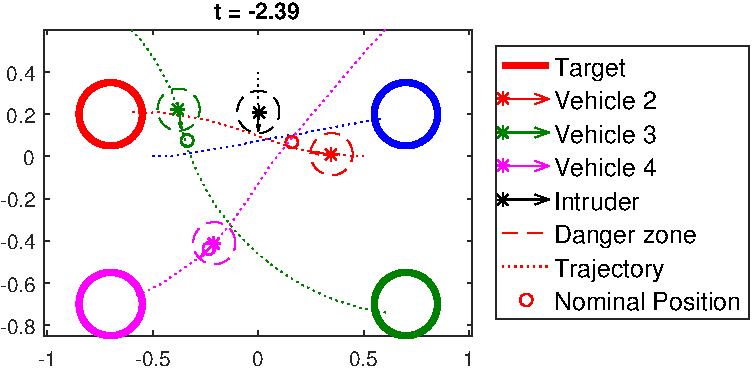
\includegraphics[width=0.9\columnwidth]{fig/intruder1_traj}
  \caption{The positions of the STP vehicles and the intruder at $t=-2.39$, the end of the intruder's appearance. The red and green vehicles $\veh_2, \veh_3$ have not been tracking their nominal trajectories for a while, and have been avoiding the intruder instead. Thus, their positions are far away from their nominal trajectories, indicated by the small colored circles. $\veh_4$ has not needed to avoid the intruder, and tracks its nominal trajectory closely. The nominal trajectory of $\veh_4$ allows it to stay far enough away from other vehicles so that all vehicles can remain safe in the presence of the intruder.}
  \label{fig:intruder1_traj}
\end{figure}

\begin{figure}
  \centering
  \includegraphics[width=\columnwidth]{"fig/intruder1_diff"}
  \caption{The difference between the initially planned nominal trajectories and the actual trajectories for vehicles $\veh_2$ (top subplot) and $\veh_3$ (bottom subplot), which needed to perform avoidance with respect to the intruder during the time interval marked by the vertical black dotted lines. Before the intruder's presence, both vehicles track their nominal trajectories closely; however, both vehicles later deviate significantly from their nominal trajectories in order to avoid the intruder. After the intruder is gone, both vehicles replan their trajectories and arrive at their targets at a later time.}
  \label{fig:intruder1_diff}
\end{figure}